% !TeX encoding = UTF-8
% !TEX root = ./presentation.tex
% !TEX spellcheck = pt_BR


\begin{frame}[fragile]{Desenvolvendo um \Wearable\ em \Software }{Construindo a Arquitetura}
\begin{figure}
    \begin{tikzpicture}[auto, node distance=4 cm, >=latex']
    %\tikzstyle{block}    = [draw, rectangle, minimum height=2em, minimum width=4em, fill=red!20]
    %\tikzstyle{input}    = [coordenate]
    %\tikzstyle{output}   = [coordenate]
    %\tikzstyle{pinstyle} = [pin edge={to-,thin,black}]
    \matrix[column sep = 2.5cm, row sep = .375cm]{
       %\node[draw, shape=rectangle, fill=red!20, visible on=<1->] (hls) {Vivado High Level Source}; &
        \node[draw, shape=rectangle, fill=red!20, visible on=<1->] (v) {Vivado}; \\
    };

    \end{tikzpicture}
    \caption{Fluxo de execução de desenvolvimento de um projeto todo em \software.}
\end{figure}
\end{frame}


\begin{frame}{Desenvolvendo um \Wearable\ em \Software }{Construindo a Arquitetura}
\vspace{-0.8em}
\begin{figure}[h] \centering
    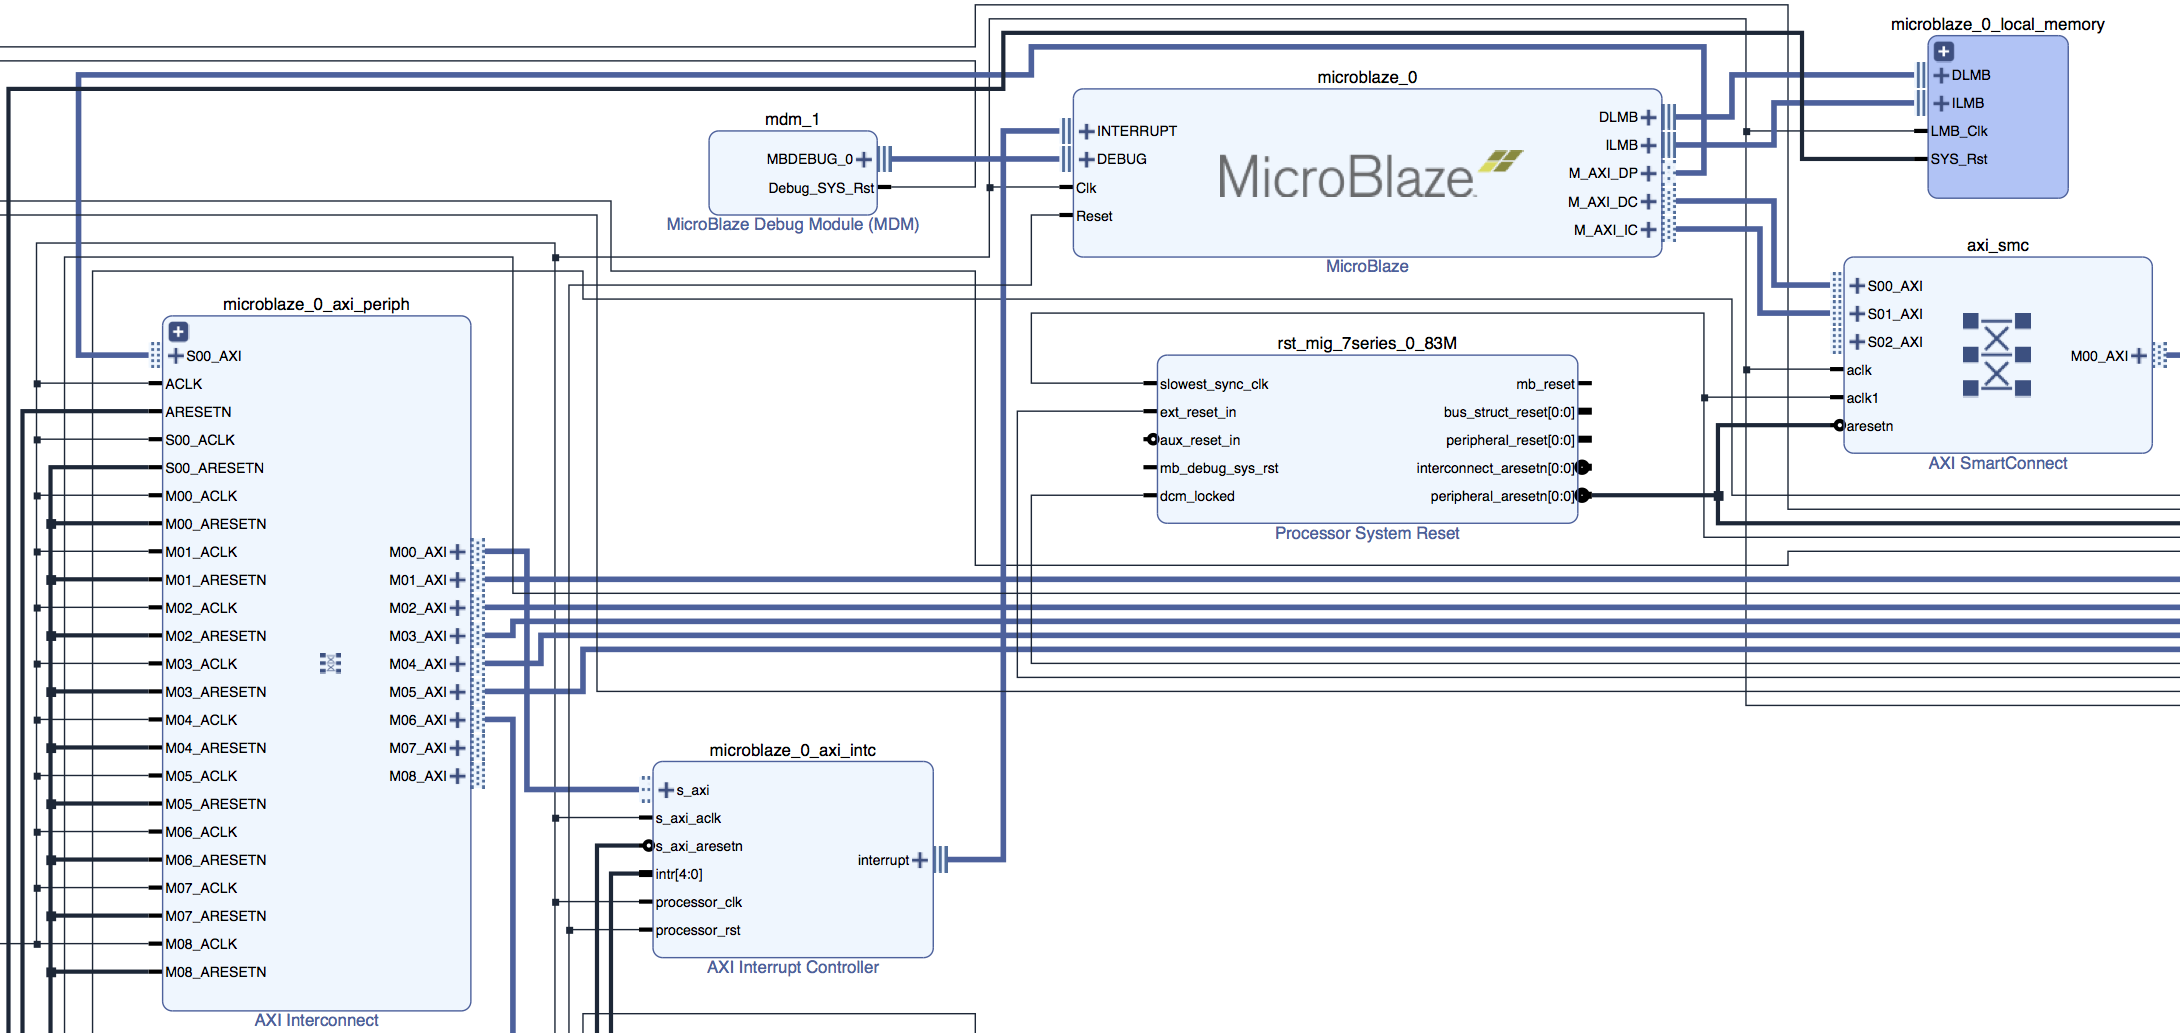
\includegraphics[width=1\textwidth]{img/vivado_software/1-microblaze-axi.png}
    \caption{Microcontrolador Microblaze e seus componentes básicos (memória e AXI).}
\end{figure}
\end{frame}

\begin{frame}{Desenvolvendo um \Wearable\ em \Software }{Construindo a Arquitetura}
\vspace{-0.8em}
\begin{figure}[h] \centering
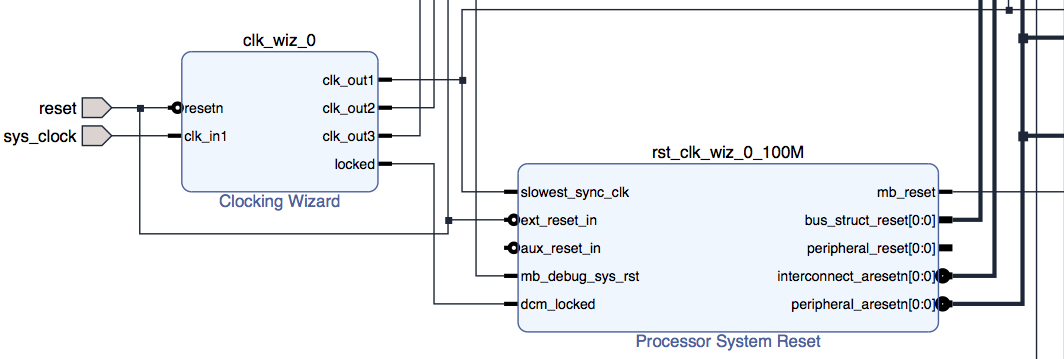
\includegraphics[width=1\textwidth]{img/vivado_software/2-clock.png}
\caption{Componentes de \textit{clock} e \textit{reset}.}
\end{figure}
\end{frame}

\begin{frame}{Desenvolvendo um \Wearable\ em \Software }{Construindo a Arquitetura}
\vspace{-1.6em}
\begin{figure}[h] \centering
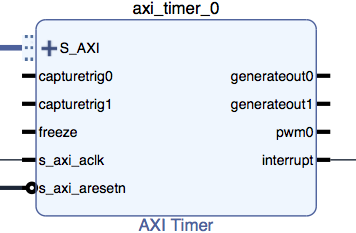
\includegraphics[width=0.4\textwidth]{img/vivado_software/3a-timer.png}
\vspace{-1em}
\caption{Componente para marcações de tempo.}
\end{figure}
\begin{figure}[h] \centering
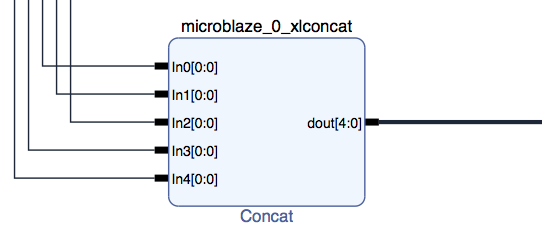
\includegraphics[width=0.67\textwidth]{img/vivado_software/3b-interruptions.png}
\vspace{-1em}
\caption{Componente para interrupções ao microcontrolador.}
\end{figure}
\end{frame}

\begin{frame}{Desenvolvendo um \Wearable\ em \Software }{Construindo a Arquitetura}
\vspace{-0.8em}
\begin{figure}[h] \centering
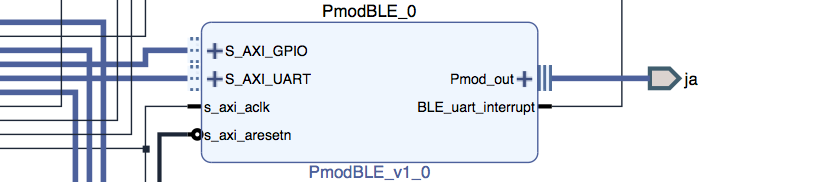
\includegraphics[width=1\textwidth]{img/vivado_software/4a-bluetooth.png}
\caption{Componente de interface do módulo bluetooth.}
\end{figure}
\begin{figure}[h] \centering
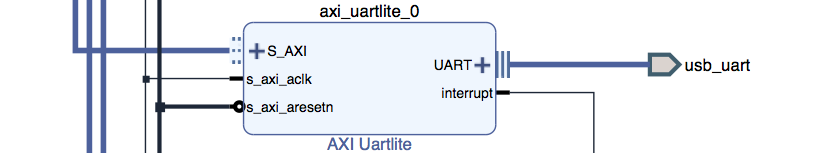
\includegraphics[width=1\textwidth]{img/vivado_software/4b-uart.png}
\caption{Componente de interface para a comunicação serial para \textit{debug}.}
\end{figure}
\end{frame}

\begin{frame}{Desenvolvendo um \Wearable\ em \Software }{Construindo a Arquitetura}
\vspace{-0.8em}
\begin{figure}[h] \centering
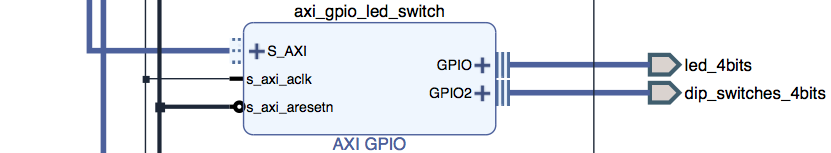
\includegraphics[width=1\textwidth]{img/vivado_software/5a-leds_switches.png}
\vspace{-1em}
\caption{Componente para acionamento \textit{leds} e leitura de \textit{switches}.}
\end{figure}
\begin{figure}[h] \centering
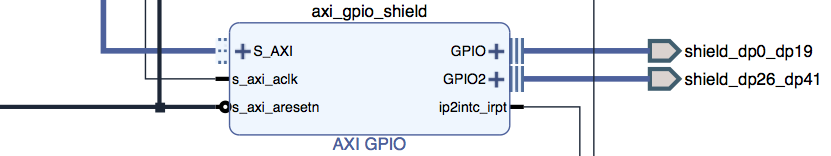
\includegraphics[width=1\textwidth]{img/vivado_software/5b-gpio.png}
\vspace{-1em}
\caption{Componente para manipulação de pinos de propósitos gerais.}
\end{figure}
\end{frame}

\begin{frame}{Desenvolvendo um \Wearable\ em \Software }{Construindo a Arquitetura - Interfaces utilizadas no \design}
\vspace{-0.8em}
\begin{figure}[h] \centering
    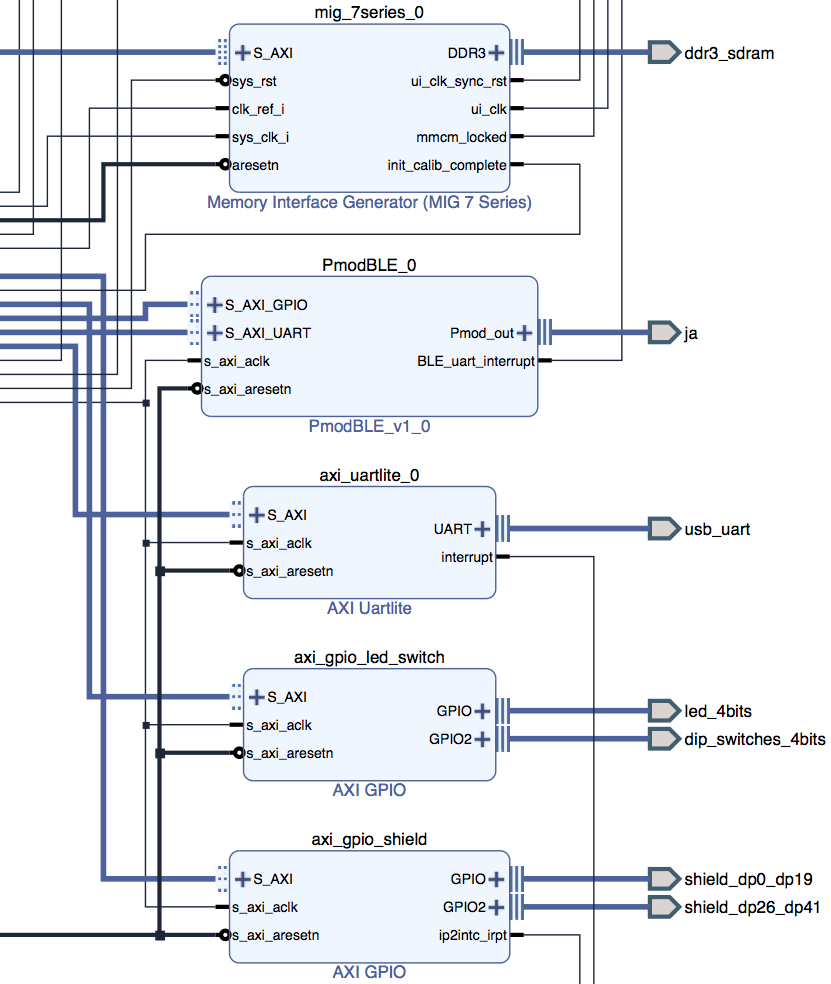
\includegraphics[width=0.55\textwidth]{img/vivado_software/6-axi_outputs.png}
    \vspace{-1em}
\end{figure}
\end{frame}

\begin{frame}{Desenvolvendo um \Wearable\ em \Software }{Construindo a Arquitetura}
\vspace{-0.8em}
\begin{figure}[h] \centering
    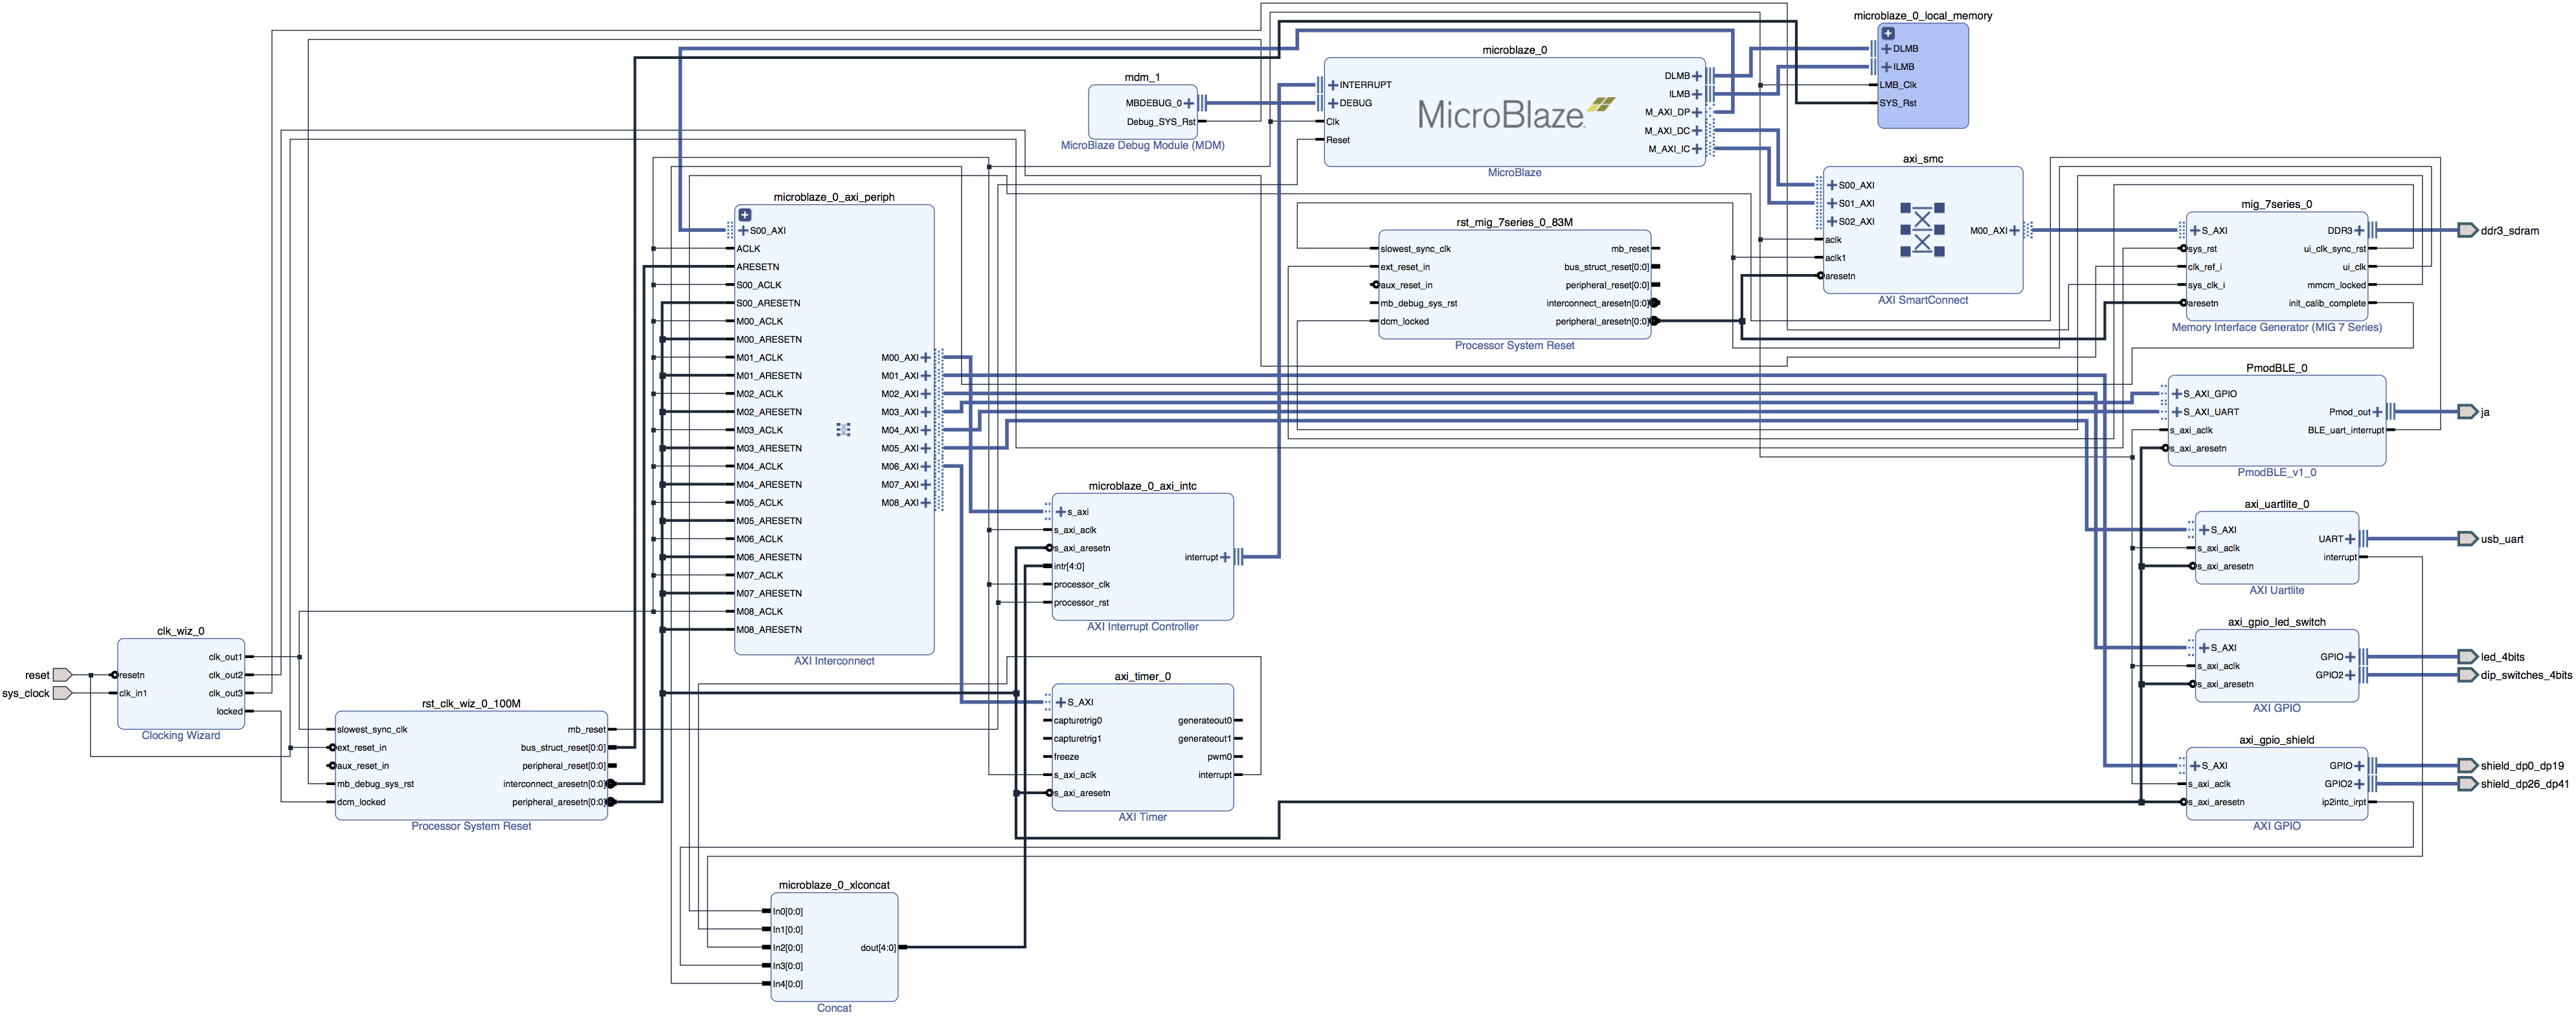
\includegraphics[width=1\textwidth]{img/vivado_software/7-all.png}
    \vspace{-1em}
    \caption{Projeto de arquitetura do sistema todo em \software .}
\end{figure}
\end{frame}

%{
%    \setbeamercolor{background canvas}{bg=}
%    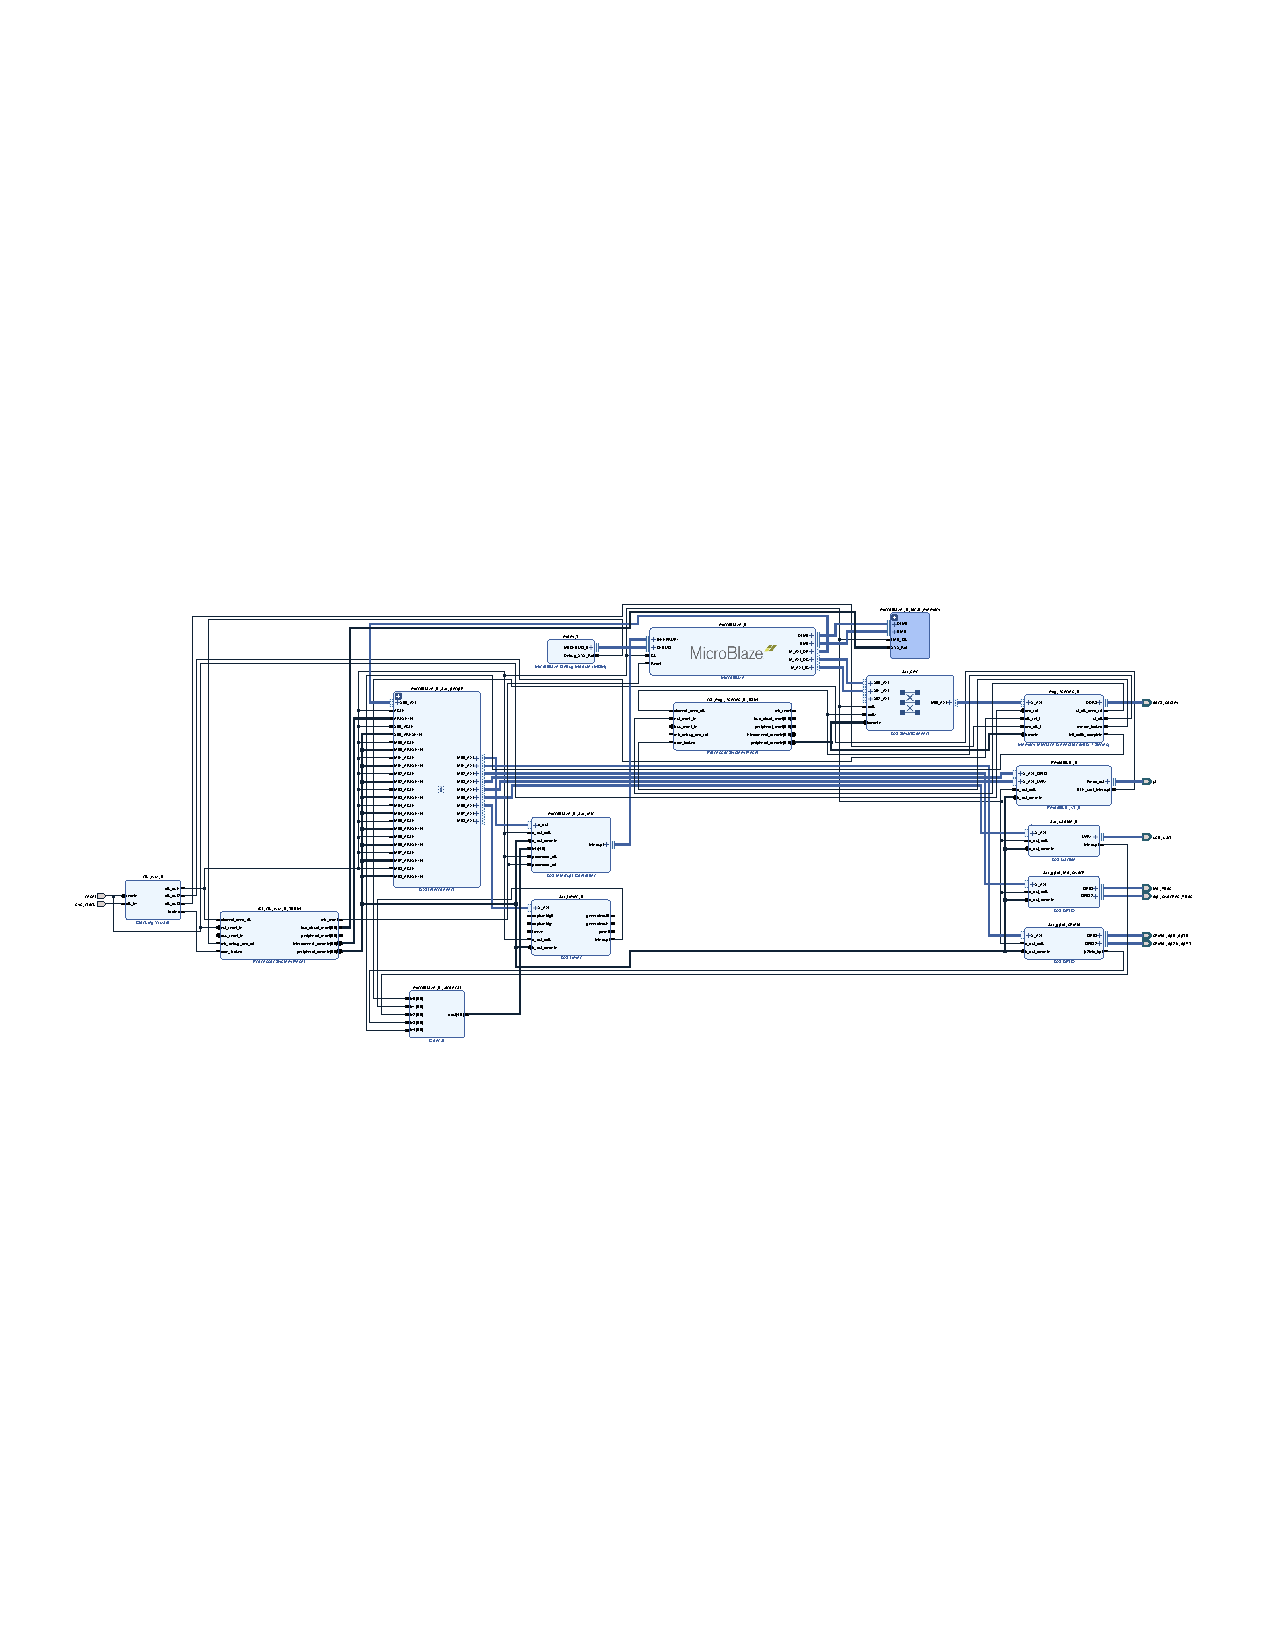
\includepdf[pages=1]{img/design.pdf}
%}


\begin{frame}[fragile]{Desenvolvendo um \Wearable\ em \Software }{Construindo o \Software }
\begin{figure}
    \begin{tikzpicture}[auto, node distance=4 cm, >=latex']
    %\tikzstyle{block}    = [draw, rectangle, minimum height=2em, minimum width=4em, fill=red!20]
    %\tikzstyle{input}    = [coordenate]
    %\tikzstyle{output}   = [coordenate]
    %\tikzstyle{pinstyle} = [pin edge={to-,thin,black}]
    \matrix[column sep = 2.5cm, row sep = .375cm]{
        %\node[draw, shape=rectangle, fill=red!20, visible on=<1->] (hls) {Vivado High Level Source}; &
        & \node[draw, shape=rectangle, fill=red!20, visible on=<1->] (v) {Vivado}; & \node[draw, shape=rectangle, fill=red!20, visible on=<2->] (sdk) {Xilinx SDK}; \\
    };
    
    \draw [->, thick, visible on=<1->] (v) -- node {export to} (sdk);
    \end{tikzpicture}
    \caption{Fluxo de execução de desenvolvimento de um projeto todo em \software.}
\end{figure}
\end{frame}


\begin{frame}{Desenvolvendo um \Wearable\ em \Software }{Construindo o \Software }
\scalebox{1}{
    \small
    \begin{algorithm}[H]
        \SetKwData{security}{security\_distance}
        \SetKwData{leds}{leds}
        \SetKwData{us}{ultrassonics}
        \SetKwData{bt}{bluetooth}
        \SetKwData{dist}{distances}
        \SetKwData{avg}{average}
        \SetKwData{variance}{variance}
        \SetKwData{sd}{standard\_derivation}
        \SetKwData{situ}{situation}

        \SetKwFunction{statmentG}{setGPIOs}
        \SetKwFunction{statmentC}{setConnections}
        \SetKwFunction{mDistance}{measure\_distance}
        \SetKwFunction{sDistance}{send\_distance}
        \SetKwFunction{safety}{vefiry\_safety}
        \SetKwFunction{evaluate}{send\_situation}

        \BlankLine
        \Begin{
            \tcp{initialyze the pins and connections}
            \statmentG{\leds, \us1..3}\;
            \statmentC{\bt}\;
            \BlankLine

            \While{is device on?}{
                \BlankLine

                \While{is bluetooth on?}{
                    \dist, \avg, \variance, \sd $\leftarrow$ \mDistance{\us1..3}\;
                    \BlankLine
                    \sDistance{\bt, \dist}\;
                    \BlankLine
                    \situ $\leftarrow$ \safety{\security, \dist}\;
                    \BlankLine
                    \evaluate{\bt, \situ}\;
                }
            }
        }

        \caption{Main Process.}
        \label{alg:wearable_main}
    \end{algorithm}
}
\end{frame}


\begin{frame}{Desenvolvendo um \Wearable\ em \Software }{Construindo o \Software }
\scalebox{1}{
    \small
    \begin{algorithm}[H]
        \SetKwData{times}{TIMES\_READ}
        \SetKwData{distance}{distances}
        \SetKwData{avg}{average}
        \SetKwData{variance}{variance}
        \SetKwData{sd}{standard\_derivation}

        \SetKwFunction{read}{read\_distance}
        \SetKwFunction{stat}{dist\_statistics}

        \BlankLine
        \Begin{

            \BlankLine
            \tcp{Read for all sensors}
            \ForEach{$s_i\ \leftarrow$ Sensors}{
                \BlankLine
                \tcp{For each sensor, read \times times}
                \For{1..\times}{
                    \distance $\leftarrow$ \read{$s_i$}\;
                }
            }

            \BlankLine

            \tcc{It calcules some statistics from data read.}
            \avg, \variance, \sd $\leftarrow$ \stat{\distance}\;

            \BlankLine

            \Return \distance, \avg, \variance, \sd
        }

        \caption{Read Distance.}
        \label{alg:wearable_read_distance}
    \end{algorithm}
}
\end{frame}

\begin{frame}[fragile, plain]{Desenvolvendo um \Wearable\ em \Software }{Construindo o Comportamento do \textit{Smartphone} }
    \vspace{-1.1em}
    \begin{center}
    \begin{minipage}{9cm}
    \begin{minted}[
    gobble=0,
    linenos,
    fontsize=\tiny,
    baselinestretch=0.9,
    numbersep=3pt,
    frame=lines]{python}

menu = read_char()
if (menu == '?'):                       # Is smartphone active?
    write_char('1')                     # Confirmation

elif (menu == 'd'):                     # Receiving distances
    write_char('1')
    quant_sensors = int(read_char())    # Number of Sesnsors

    write_char('1')
    distances = []
    variances = []
    sds       = []
    for i in range(0, quant_sensors):
        distance = '0'                  # First distance
        number = read_char()
        while (number != 'e'):
            distance += number
            number = read_char()
        distances.append(distance)

        variance = '0'                  # Second variance
        number = read_char()
        while (number != 'e'):
            variance += number
            number = read_char()
        variances.append(variance)

        sd = '0'                        # Third standard derivation
        number = read_char()
        while (number != ';'):
            sd += number
            number = read_char()
            sds.append(sd)

elif (menu == 's'):                     # Receiving the wearable's situation
    situation = read_char()
    write_char('1')
    \end{minted}
\end{minipage}
\end{center}
\end{frame}


\begin{frame}{Protótipo}
\vspace{-0.8em}
\begin{figure}[h] \centering
    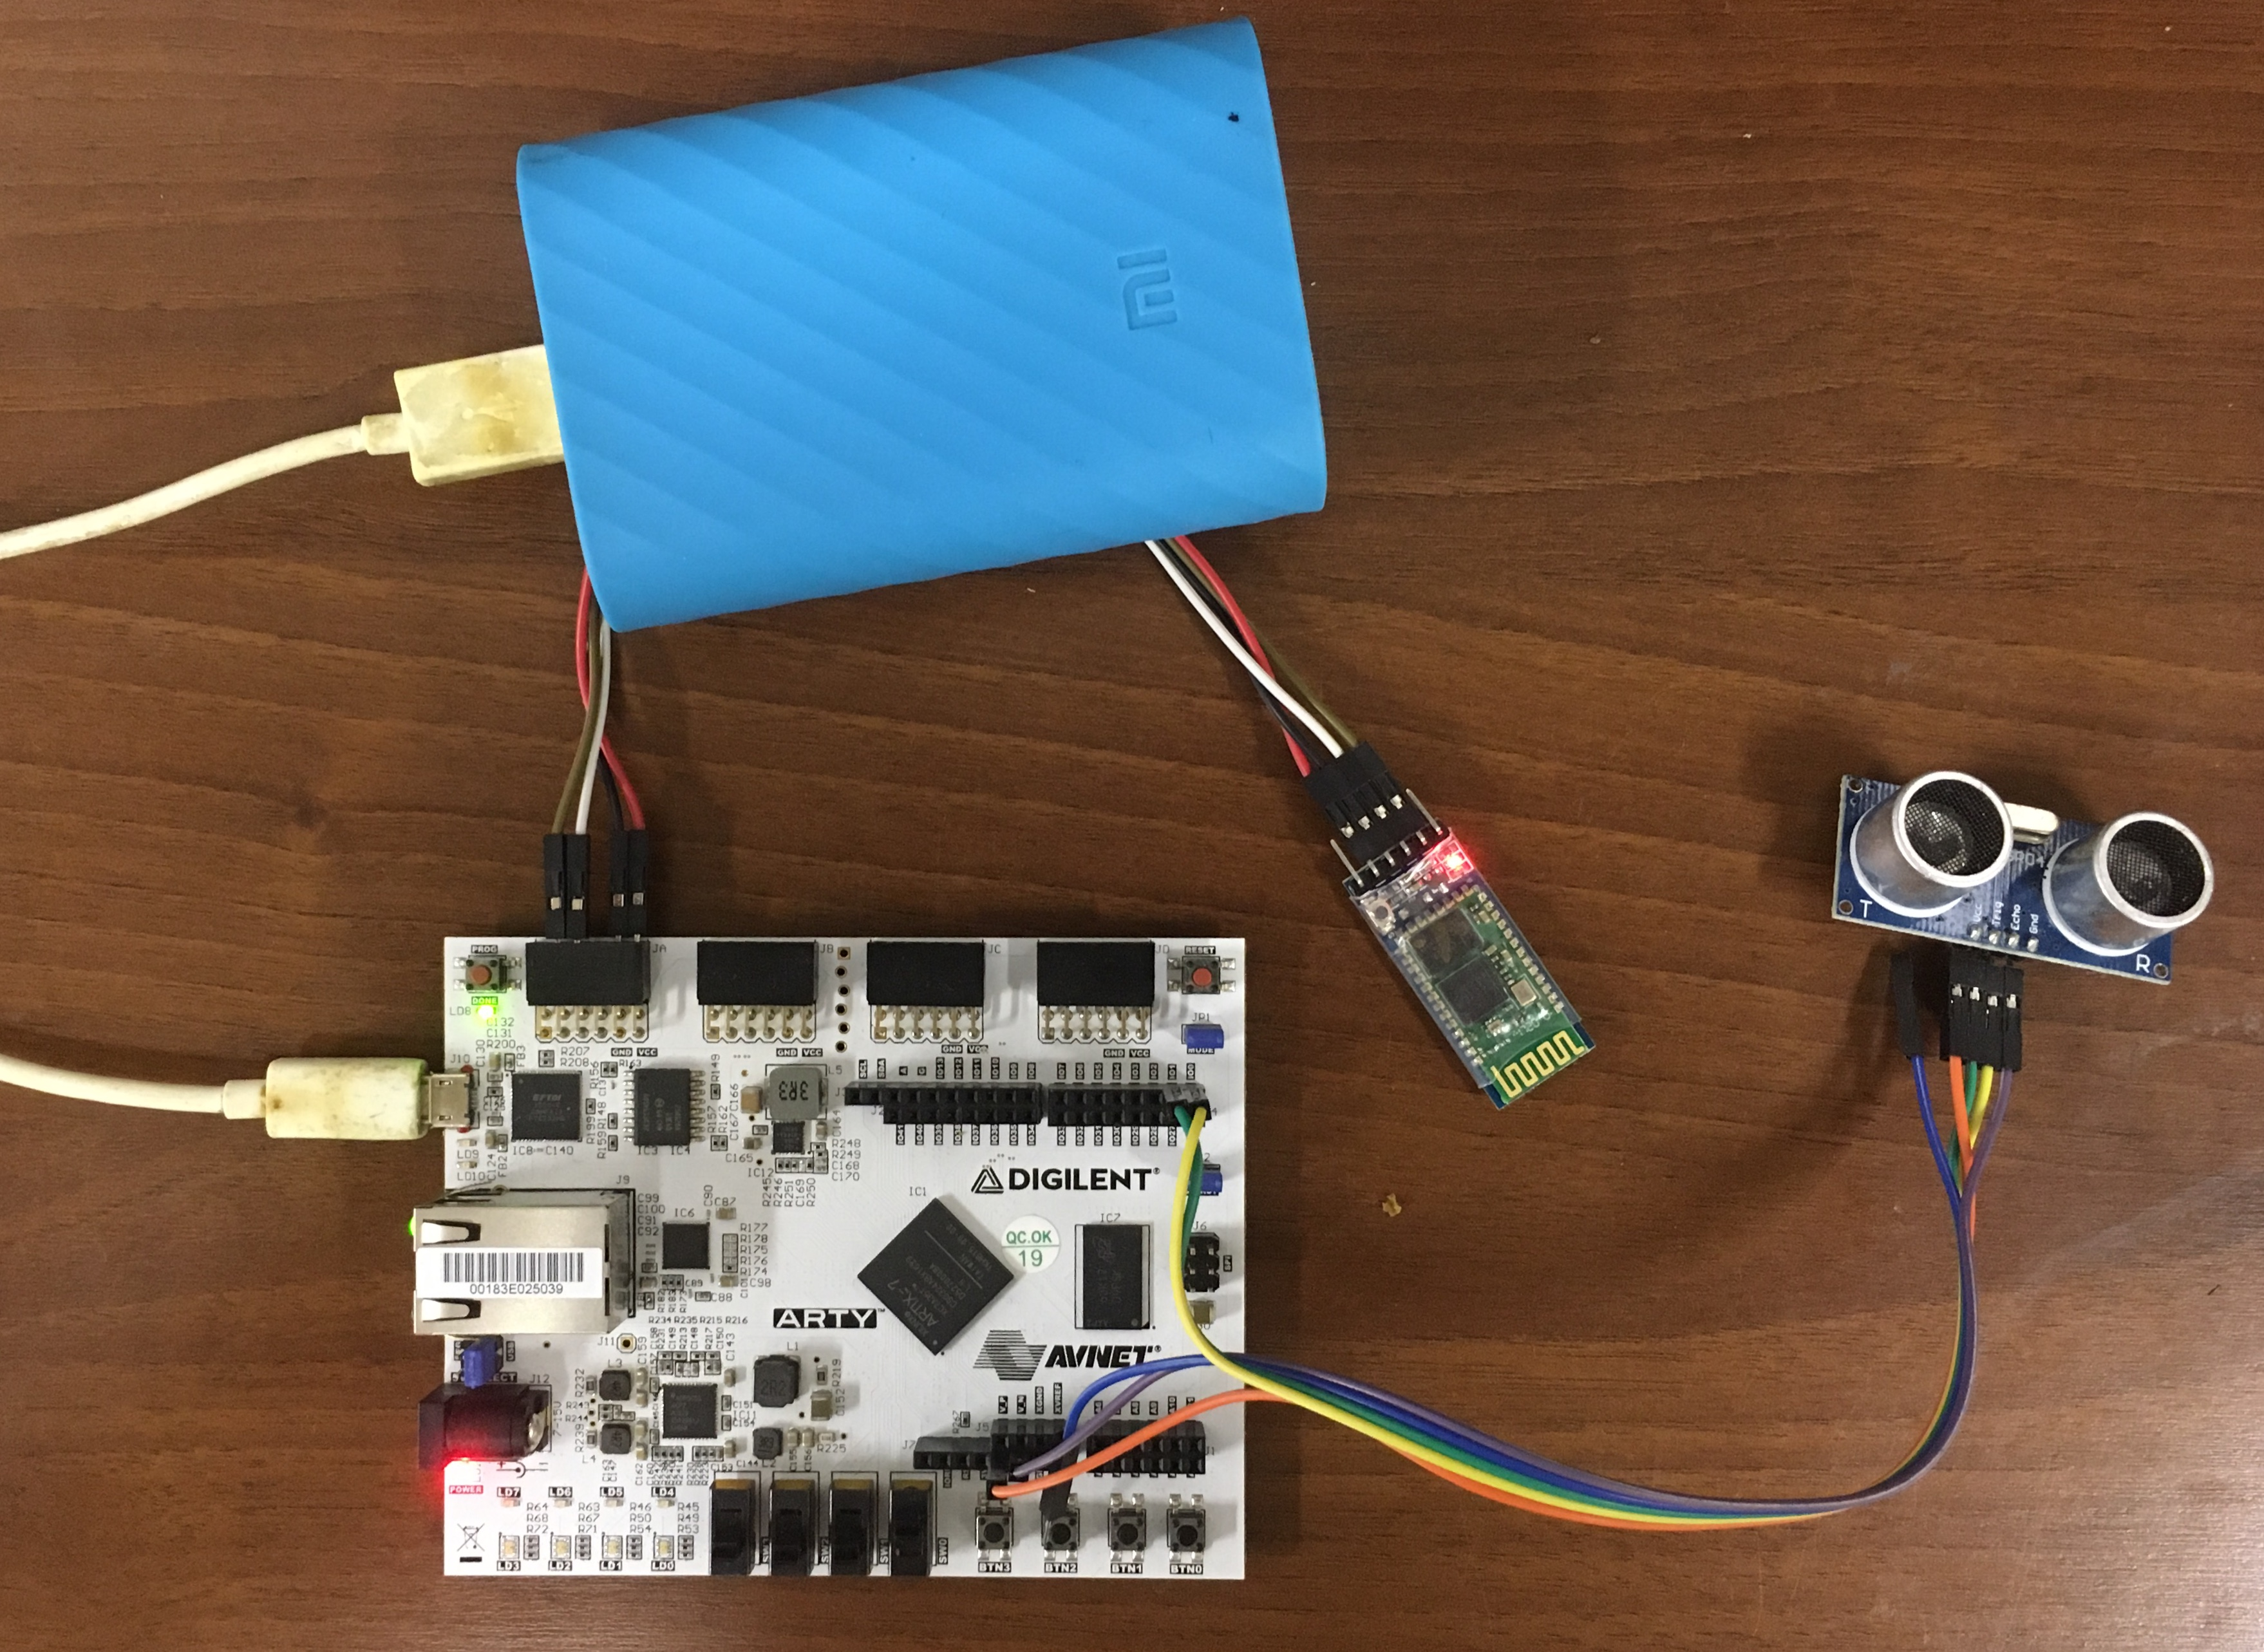
\includegraphics[width=0.9\textwidth]{img/placa.jpg}
    \vspace{-1em}
    \caption{Protótipo utilizado.}
\end{figure}
\end{frame}

\begin{frame}{Desenvolvendo um \Wearable\ em \Software }
\vspace{-0.8em}
\begin{figure}[h] \centering
    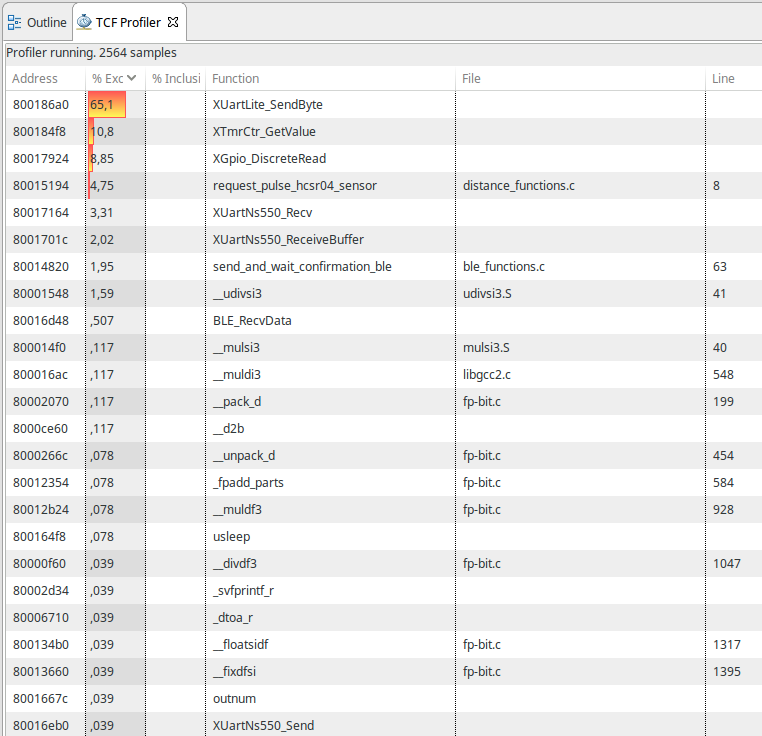
\includegraphics[width=0.68\textwidth]{img/tcf_software.png}
    \vspace{-1em}
    \caption{\Profile\ do projeto em \software .}
\end{figure}
\end{frame}


\begin{frame}[fragile]{Desenvolvendo um \Wearable\ em \Hardware }{Metodologia de Desenvolvimento}
\begin{figure}
    \begin{tikzpicture}[auto, node distance=4 cm, >=latex']
    %\tikzstyle{block}    = [draw, rectangle, minimum height=2em, minimum width=4em, fill=red!20]
    %\tikzstyle{input}    = [coordenate]
    %\tikzstyle{output}   = [coordenate]
    %\tikzstyle{pinstyle} = [pin edge={to-,thin,black}]
    \matrix[column sep = 2.8cm, row sep = .375cm]{
        \node[draw, shape=rectangle, fill=red!20, visible on=<2->] (hls) {Vivado HLS}; & \node[draw, shape=rectangle, fill=red!20, visible on=<1->] (v) {Vivado}; & \node[draw, shape=rectangle, fill=red!20, visible on=<1->] (sdk) {Xilinx SDK}; \\
    };

    \draw [->, thick, visible on=<1->] (v) -- node {export to} (sdk);
    \draw [dashed, ->, thick, visible on=<2->] (hls) -- node {new hardware} (v);
    \end{tikzpicture}
    \caption{Fluxo de execução de desenvolvimento de um projeto com módulos em \hardware.}
\end{figure}
\end{frame}


\begin{frame}{Desenvolvendo um \Wearable\ em \Hardware }{Algoritmo a ser Particionado}
\scalebox{1}{
    \small
    \begin{algorithm}[H]
        \SetKwData{times}{TIMES\_READ}
        \SetKwData{distance}{distances}
        \SetKwData{avg}{average}
        \SetKwData{variance}{variance}
        \SetKwData{sd}{standard\_derivation}
        
        \SetKwFunction{read}{read\_distance}
        \SetKwFunction{stat}{dist\_statistics}
        
        \BlankLine
        \Begin{
            
            \BlankLine
            \tcp{Read for all sensors}
            \ForEach{$s_i\ \leftarrow$ Sensors}{
                \BlankLine
                \tcp{For each sensor, read \times times}
                \For{1..\times}{
                    \distance $\leftarrow$ \read{$s_i$}\;
                }
            }
            
            \BlankLine
            
            \tcc{It calcules some statistics from data read.}
            \avg, \variance, \sd $\leftarrow$ \stat{\distance}\;
            
            \BlankLine
            
            \Return \distance, \avg, \variance, \sd
        }
        
        \caption{Read Distance.}
        \label{alg:wearable_read_distance2}
    \end{algorithm}
}
\end{frame}

\begin{frame}[fragile, plain]{Desenvolvendo um \Wearable\ em \Hardware }{Algoritmo a ser Particionado}
\vspace{-0.6em}
\begin{center}
    \begin{minipage}{10cm}
        \begin{minted}[
        gobble=0,
        linenos,
        fontsize=\tiny,
        baselinestretch=1.1,
        numbersep=8pt,
        frame=lines]{c}
#define TIMES_MEASURES 5

void calcule_stats(float v[TIMES_MEASURES], float * avg, float * variance, float * sd)
{
#pragma HLS INTERFACE s_axilite port=v        register bundle=BUS_AXILiteS depth=5
#pragma HLS INTERFACE s_axilite port=avg      register bundle=BUS_AXILiteS
#pragma HLS INTERFACE s_axilite port=variance register bundle=BUS_AXILiteS
#pragma HLS INTERFACE s_axilite port=sd       register bundle=BUS_AXILiteS
#pragma HLS INTERFACE s_axilite port=return            bundle=BUS_AXILiteS

    float sum = 0;
    int i = 0;

    // Searches for the max and min values
    forSum: for (i = 0; i < TIMES_MEASURES; i++) {
        sum += v[i];
    }

    // Calcules the avg
    *avg = sum / (TIMES_MEASURES);


     // Variances
    forVariance: for (i = 0; i < TIMES_MEASURES; i++) {
        *variance += (v[i] - *avg) * (v[i] - *avg);
    }

    *variance /= TIMES_MEASURES;

    *sd = sqrt(*variance);
}
        \end{minted}
    \end{minipage}
\end{center}
\end{frame}


\begin{frame}{Desenvolvendo um \Wearable\ em \Hardware }{Acoplamento à Arquitetura}
\vspace{-0.8em}
\begin{figure}[h] \centering
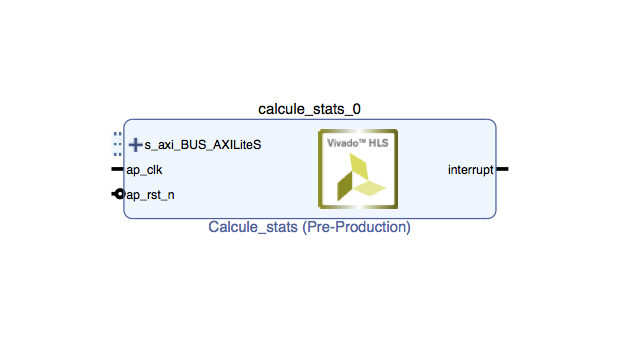
\includegraphics[width=1\textwidth]{img/vivado_hardware/desligado.png}
\vspace{-1em}
\caption{Projeto de arquitetura do sistema todo em \hardware.}
\end{figure}
\end{frame}

\begin{frame}{Desenvolvendo um \Wearable\ em \Hardware }{Acoplamento à Arquitetura}
\vspace{-0.8em}
\begin{figure}[h] \centering
    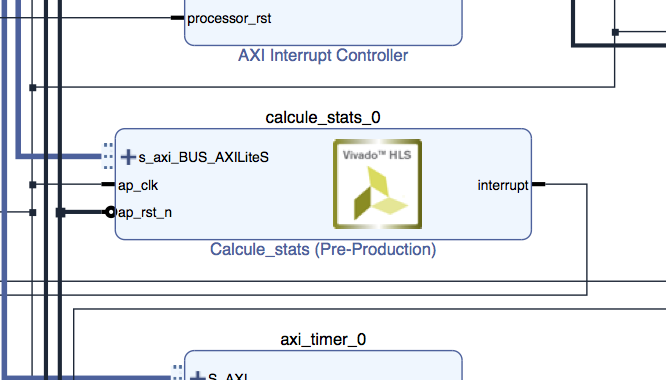
\includegraphics[width=1\textwidth]{img/vivado_hardware/ligado.png}
    \vspace{-1em}
    \caption{Projeto de arquitetura do sistema todo em \hardware.}
\end{figure}
\end{frame}


\begin{frame}{Desenvolvendo um \Wearable\ em \Hardware }{Acoplamento à Arquitetura}
\vspace{-0.8em}
\begin{figure}[h] \centering
    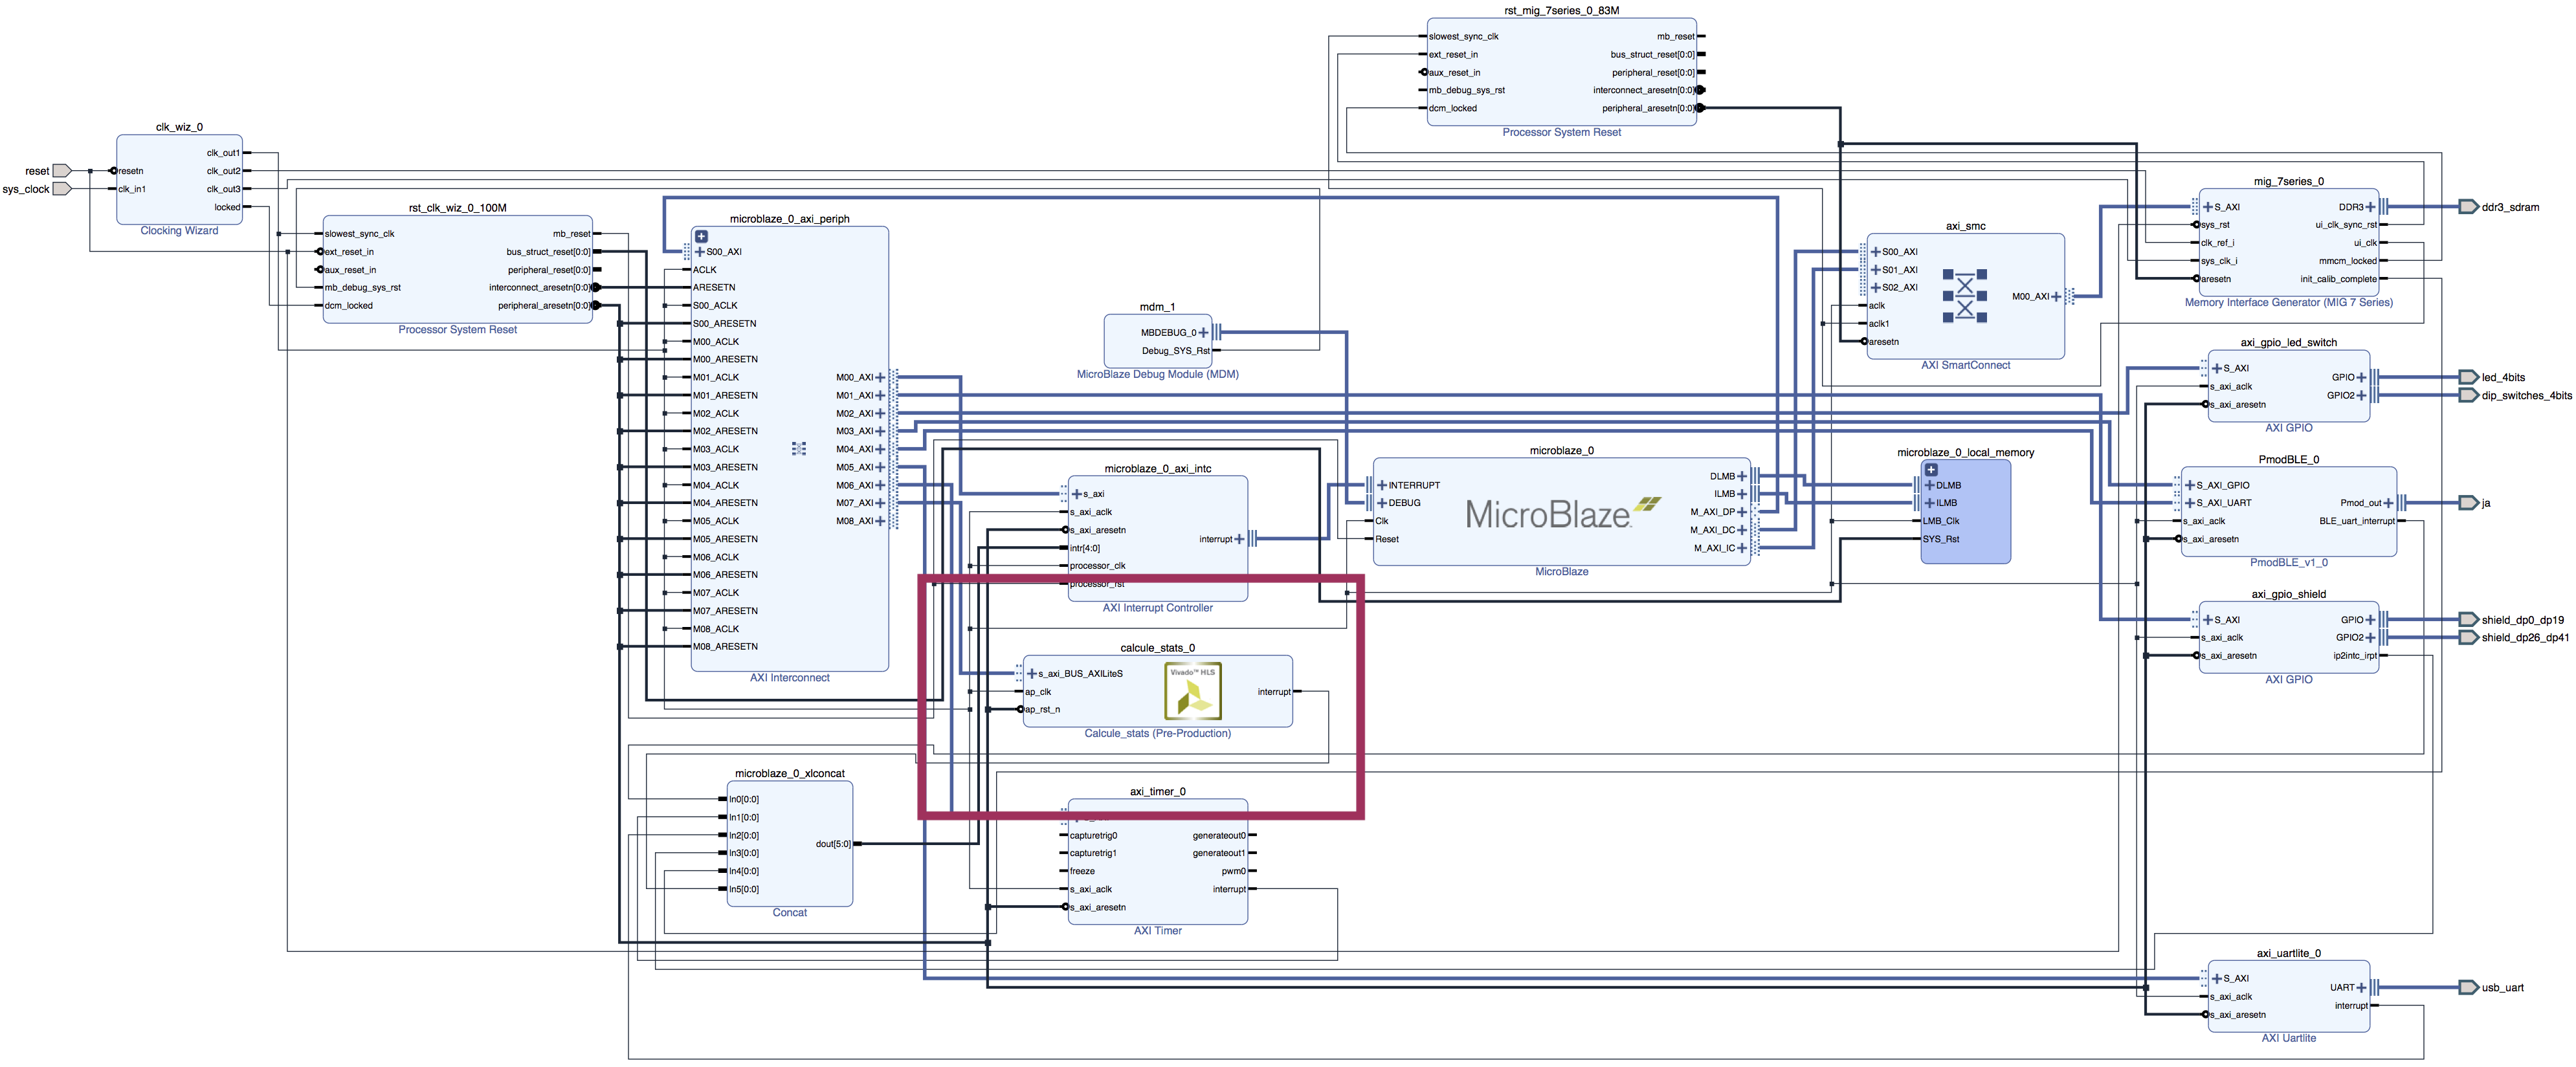
\includegraphics[width=1\textwidth]{img/vivado_hardware/all.png}
    \vspace{-1em}
    \caption{Projeto de arquitetura do sistema todo em \hardware.}
\end{figure}
\end{frame}


\begin{frame}{Situações para Teste}

\begin{table}\centering
    \scriptsize
    \raaa{1.3}
    \caption{Cálculo de performance sobre variações em I/O e algoritmo particionado.}
    \begin{tabular}{@{}rrrrcrrrcrrr@{}}\toprule
        & \multicolumn{3}{c}{$\mathcal{O}(1)$} && \multicolumn{3}{c}{$\mathcal{O}(n)$} & & \multicolumn{3}{c}{$\mathcal{O}(n\log n)$}\\
        \cmidrule{2-4} \cmidrule{6-8} \cmidrule{10-12}análise& $s=0$ & $s=1$ & $s=2$ && $s=0$ & $s=1$ & $s=2$ &&$s=0$ & $s=1$ & $s=2$ \\
        \midrule \textit{sistêmica} \\
        %média     & ? & ? & ? && ? & ? & ? && ? & ? & ? \\
        $\bar{x}$     & ? & ? & ? && ? & ? & ? && ? & ? & ? \\
        $\sigma^2$ & ? & ? & ? && ? & ? & ? && ? & ? & ? \\
        $\sigma$ & ? & ? & ? && ? & ? & ? && ? & ? & ? \\
        \midrule \textit{empírica} \\
        %média     & ? & ? & ? && ? & ? & ? && ? & ? & ? \\
        $\bar{x}$     & ? & ? & ? && ? & ? & ? && ? & ? & ? \\
        $\sigma^2$ & ? & ? & ? && ? & ? & ? && ? & ? & ? \\
        $\sigma$ & ? & ? & ? && ? & ? & ? && ? & ? & ? \\
        \bottomrule
    \end{tabular}
\end{table}
\end{frame}